\section{Comparación de Algoritmos y Escalamiento}
\label{sec:comparacion_escalamiento}

\subsection{Comparación Global de Rendimiento}
En esta sección se comparan exhaustivamente las tres variantes evaluadas para $N=2048$:
\begin{itemize}
    \item \textbf{Algoritmo 1 (C++ OpenMP):} Paralelismo de datos plano con \texttt{\#pragma omp parallel for schedule(static)}.
    \item \textbf{Algoritmo 2 (C++ OpenMP):} Dividir y conquistar recursivo con paralelismo de tareas (\texttt{\#pragma omp task}) y tamaño de bloque base $n=256$.
    \item \textbf{Algoritmo 3 (Python Numba):} Paralelismo de datos compilado JIT mediante \texttt{@njit(parallel=True)} y \texttt{prange}.
\end{itemize}

La Figura~\ref{fig:exp_e_comparacion} presenta las curvas de tiempo de ejecución $T(p)$, \emph{speedup} $S(p)$ y eficiencia paralela $E(p)$ para ambas máquinas frente a la referencia ideal de escalamiento lineal ($S_{\text{ideal}}=p$, $E_{\text{ideal}}=1.0$).

\begin{figure}[htbp]
    \centering
    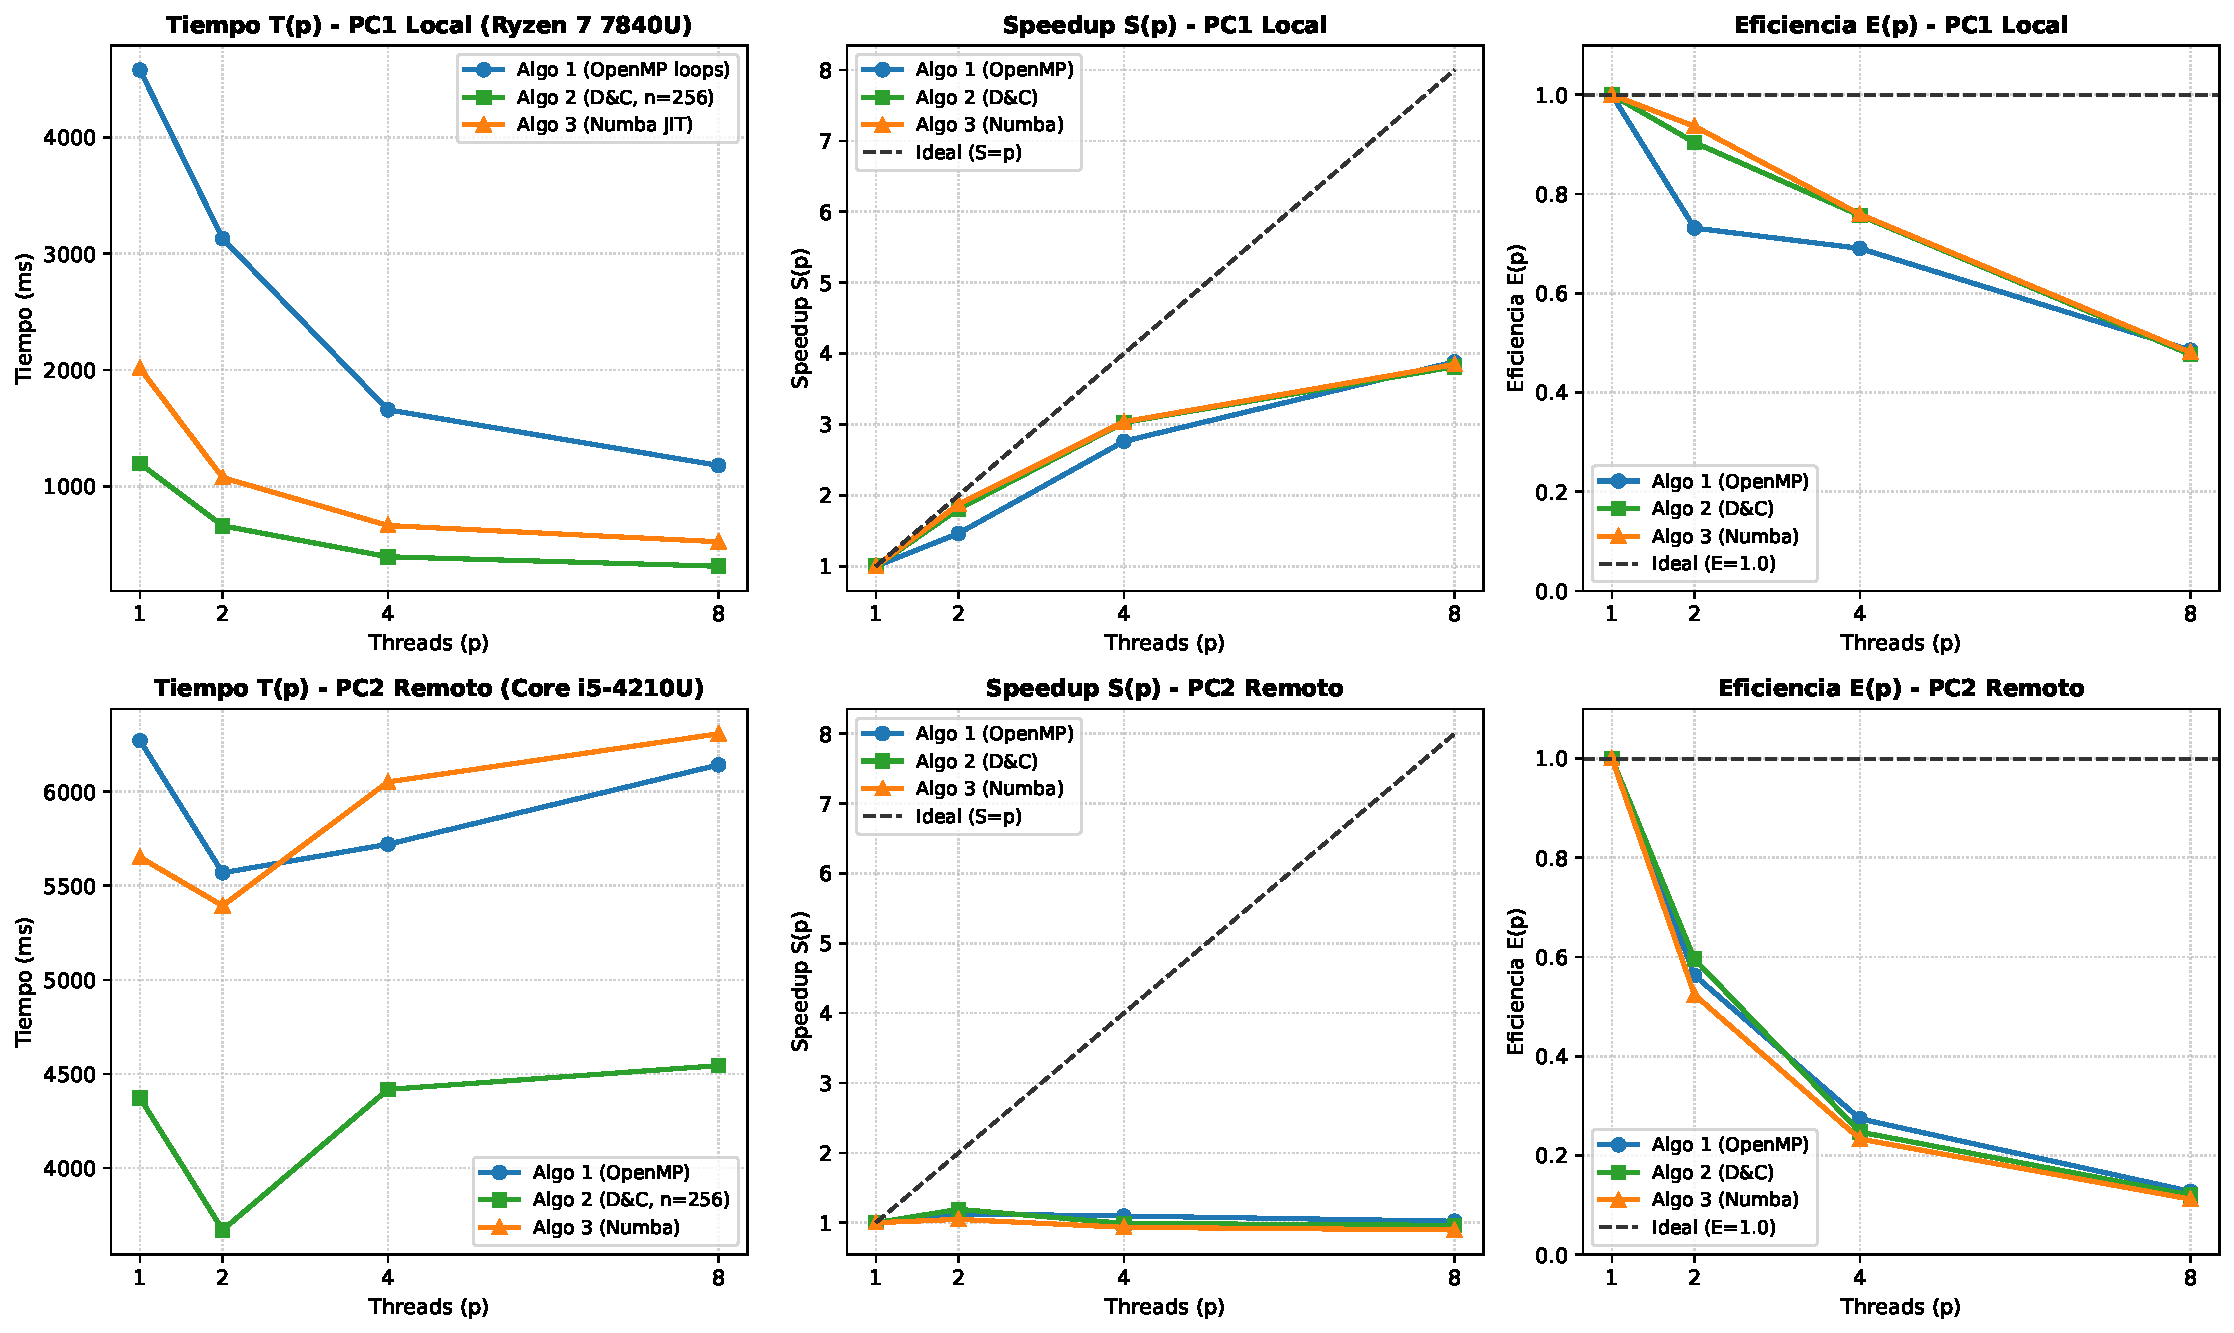
\includegraphics[width=\textwidth]{E/exp_e_comparacion.pdf}
    \caption{Comparación de $T(p)$, $S(p)$ y $E(p)$ entre los tres algoritmos frente a la curva ideal en PC1 Local (Ryzen 7 7840U) y PC2 Remoto (Core i5-4210U).}
    \label{fig:exp_e_comparacion}
\end{figure}

Del análisis comparativo se desprenden tres conclusiones esenciales:
\begin{enumerate}
    \item \textbf{Supremacía del Algoritmo 2 en tiempo absoluto:} En PC1, el Algoritmo 2 supera con holgura a las demás versiones en todas las configuraciones, registrando apenas \SI{313.49}{\milli\second} a 8 hilos (frente a \SI{523.67}{\milli\second} de Numba y \SI{1179.62}{\milli\second} del Algoritmo 1). Este resultado demuestra que el aprovechamiento de la jerarquía de memoria caché mediante particionamiento en bloques supera a cualquier paralelización de bucles planos sobre matrices que desbordan la memoria caché.
    \item \textbf{Eficiencia de Numba frente a C++ estándar:} En PC1, el Algoritmo 3 en Python con Numba es consistentemente más del doble de rápido que el Algoritmo 1 en C++ (\SI{2014.47}{\milli\second} vs \SI{4579.82}{\milli\second} en $p=1$, y \SI{523.67}{\milli\second} vs \SI{1179.62}{\milli\second} en $p=8$). La generación de código nativo vía LLVM en Numba aplica vectorización SIMD agresiva (AVX2/FMA) sobre las acumulaciones internas, superando la compilación directa de bucles anidados en C++.
    \item \textbf{Saturación de hardware en PC2:} En el procesador Intel Core i5 de bajo consumo (15W TDP, 2 cores), todas las versiones se estancan a partir de $p \ge 2$. La falta de núcleos físicos adicionales y el sobrecalentamiento impiden obtener ganancias paralelas significativas.
\end{enumerate}

\subsection{Justificación de la Elección de $T(1)$}
Para cuantificar el \emph{speedup} $S(p) = T(1)/T(p)$ y la eficiencia $E(p) = S(p)/p$, surgen dos alternativas formales para fijar la base $T(1)$:
\begin{enumerate}
    \item \textbf{Speedup Relativo ($T(1) = T_{\text{alg}}(1)$):} Se normaliza respecto al tiempo del propio algoritmo ejecutado con un único hilo.
    \item \textbf{Speedup Absoluto ($T(1) = T_{\text{serial}}$):} Se normaliza respecto al mejor tiempo secuencial absoluto de referencia (por ejemplo, el caso base óptimo en \texttt{serial.cpp} o el Algoritmo 2 con 1 hilo).
\end{enumerate}

\textbf{Justificación:} En este trabajo se adoptó el \textbf{Speedup Relativo} en los gráficos principales con el fin de evaluar de forma aislada la \emph{escalabilidad intrínseca} y el costo de gestión concurrente de cada runtime (el scheduler estático de OpenMP, el despachador de tareas de OpenMP y el pool de hilos de Numba), sin penalizar a los algoritmos por diferencias de rendimiento puramente secuenciales.

No obstante, la comparación con el gráfico de tiempo absoluto $T(p)$ es imprescindible: aunque el Algoritmo 1 muestra un speedup relativo de $3.88\times$ en $p=8$ (aparentemente superior al $3.81\times$ del Algoritmo 2), el Algoritmo 2 con \textbf{un solo hilo} (\SI{1195.60}{\milli\second}) es prácticamente tan rápido como el Algoritmo 1 con \textbf{ocho hilos} (\SI{1179.62}{\milli\second}). El speedup relativo puede ser engañoso si se analiza de forma aislada.

\subsection{Efecto del Tamaño de Bloque $n$ en el Algoritmo 2}
Para responder al requerimiento del enunciado sobre cómo cambia el resultado al variar el tamaño de bloque, se realizó un barrido experimental en PC1 variando $n \in \{64, 128, 256, 512, 1024\}$ para cada concurrencia $p \in \{1, 2, 4, 8\}$. Los resultados se presentan en la Figura~\ref{fig:exp_e_algo2_bloques} y en la Tabla~\ref{tab:algo2_sweep}.

\begin{figure}[htbp]
    \centering
    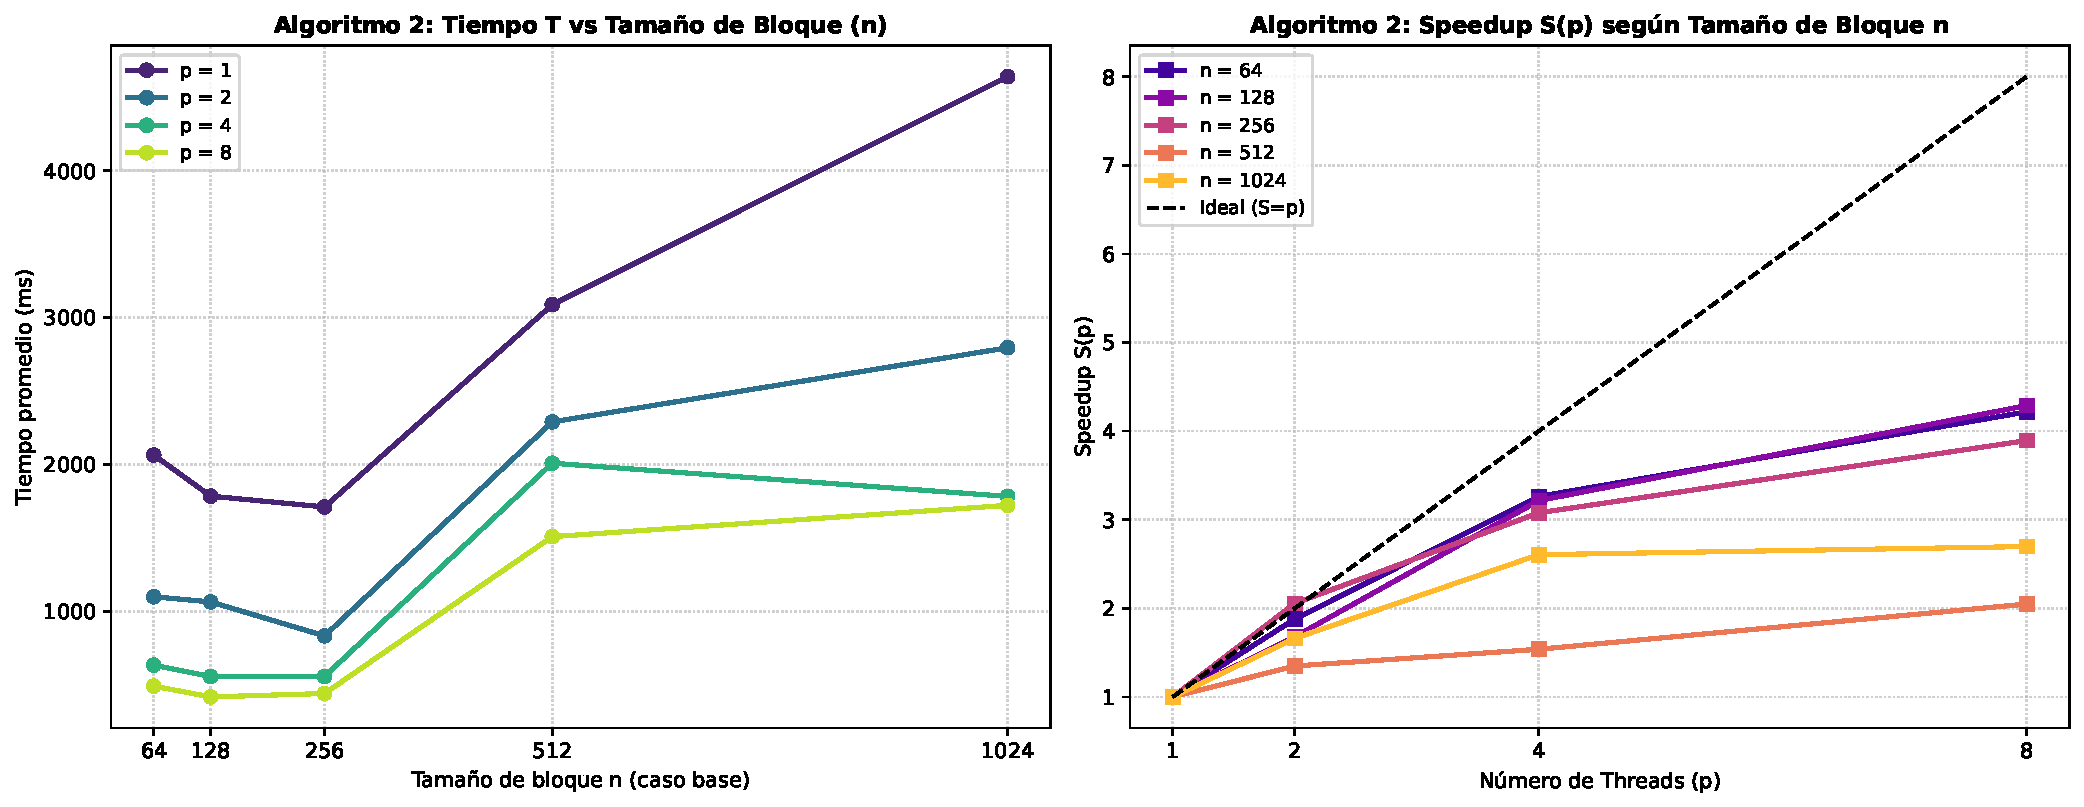
\includegraphics[width=\textwidth]{E/exp_e_algo2_bloques.pdf}
    \caption{Impacto del tamaño de bloque $n$ en el Algoritmo 2: Tiempo de ejecución $T(n)$ por número de hilos (izquierda) y escalamiento de Speedup $S(p)$ según $n$ (derecha).}
    \label{fig:exp_e_algo2_bloques}
\end{figure}

\begin{table}[htbp]
\centering
\footnotesize
\setlength{\tabcolsep}{5pt}
\caption{Tiempos promedio (ms), Speedup $S(p)$ y Eficiencia $E(p)$ del Algoritmo 2 según $n$ y $p$ en PC1 Local.}
\label{tab:algo2_sweep}
\begin{tabular}{r ccc ccc}
\toprule
$n$ & $p=1$ (ms) & $p=2$ (ms) & $p=4$ (ms) & $p=8$ (ms) & $S(8)$ & $E(8)$ \\
\midrule
64   & 2063.60 & 1098.02 & 632.58 & 489.35 & 4.22 & 0.53 \\
128  & 1783.67 & 1062.88 & 554.73 & 415.92 & 4.29 & 0.54 \\
256  & 1709.87 &  831.81 & 555.59 & 439.21 & 3.89 & 0.49 \\
512  & 3087.74 & 2289.18 & 2008.05 & 1507.67 & 2.05 & 0.26 \\
1024 & 4641.30 & 2794.67 & 1781.82 & 1720.91 & 2.70 & 0.34 \\
\bottomrule
\end{tabular}
\end{table}

\subsection{Análisis del Comportamiento según $n$}
\begin{enumerate}
    \item \textbf{Curva en U del tiempo de ejecución:} Para todo número de hilos $p$, el tiempo sigue un perfil convexo con un óptimo claro en $n=128$ y $n=256$.
    \item \textbf{Degradación con bloques grandes ($n \ge 512$):} Con $n=1024$, cada cuadrante ocupa 8 MiB, superando la caché L2 privada de cada núcleo (1 MiB) y saturando los accesos a memoria. Adicionalmente, el árbol se detiene tras una sola subdivisión, generando únicamente 4 tareas. Al haber 8 hilos y solo 4 tareas, 4 núcleos quedan completamente desocupados (\emph{task starvation}), provocando un speedup bajo ($2.70\times$ en $p=8$).
    \item \textbf{Degradación por sobrecarga con bloques pequeños ($n=64$):} Aunque un bloque de $64 \times 64$ (32 KiB) cabe holgadamente en la caché L1 de datos, genera $(2048/64)^2 = 1024$ tareas hoja y 6 niveles de llamadas. El costo administrativo del planificador de tareas de OpenMP incrementa el tiempo absoluto en comparación con $n=128$ y $n=256$.
    \item \textbf{Zona óptima de compromiso ($n \in [128, 256]$):} Estos tamaños ofrecen el balance óptimo: generan entre 64 y 256 tareas independientes (suficientes para balancear la carga entre 8 núcleos) mientras los bloques de trabajo caben dentro de la caché L2 rápida, logrando los tiempos de ejecución mínimos absolutos.
\end{enumerate}
